% HiMCM 2022 Problem A --- The Need for Bees
% Compile from this directory:
%   pdflatex himcm_paper.tex && pdflatex himcm_paper.tex
% Figures: ../paper_figures/   Tables: numbers from ../results/*.csv only.
\documentclass[12pt]{article}

\usepackage[margin=1in]{geometry}
\usepackage{amsmath,amssymb,amsfonts}
\usepackage{booktabs}
\usepackage{graphicx}
\usepackage{caption}
\usepackage{subcaption}
\usepackage{setspace}
\usepackage{enumitem}
\usepackage{array}
\usepackage{multirow}
\usepackage[hidelinks]{hyperref}

\graphicspath{{../paper_figures/}{paper_figures/}{./}}
\hypersetup{
  pdftitle={HiMCM 2022 Problem A: The Need for Bees},
  pdfauthor={Team XXXX}
}

\newcommand{\TeamNumber}{XXXX}
\newcommand{\Lmax}{L_{\max}}
\newcommand{\muF}{\mu_{F}}
\newcommand{\etaN}{\eta_{N}}
\newcommand{\etaP}{\eta_{P}}
\newcommand{\sigF}{\sigma_{F}}

\pagestyle{myheadings}
\markright{\TeamNumber \hfill HiMCM 2022 Problem A \hfill}

\title{\textbf{Dual-Feedback Honeybee Dynamics, Differentiable Sensitivity,\\
and Pollination Capacity on a 20-Acre Almond Farm}\\[0.4em]
\large HiMCM 2022 Problem A --- Team \TeamNumber}
\author{}
\date{}

\begin{document}
\maketitle
\thispagestyle{empty}

\begin{center}
{\Large \textbf{Summary}}
\end{center}

\noindent
We build a five-compartment dual-feedback colony model
\(y=[B,H,F,P,N]\) (brood, hive bees, foragers, pollen stores, nectar stores)
with \(C^\infty\) activations (Holling-III, Softplus projection, seasonal
\(\Omega(t)\)). A PyTorch Euler rollout
(\texttt{DifferentiableColonySimulator}) yields year-long trajectories under
a healthy baseline and a field triple-stress protocol (pesticide, Varroa,
late frost).

\underline{Healthy baseline} (\texttt{ccd\_healthy\_vs\_stress\_snapshot.csv}):
summer peak adults \(H+F=66{,}507\) (day 238); overwinter adults
\(38{,}622\). Under field stress at \(\muF=0.28\), the same metric falls to
a summer peak of \(5{,}630\) and overwinter \(3{,}163\).

\underline{Autograd elasticities}
(\texttt{autograd\_elasticity\_ranking.csv}) for
\(J_{\mathrm{pop}}=H+F\) at day 365 rank
\(\Lmax\) (\(S=+0.925\)), \(\muF\) (\(S=-0.311\)), and social inhibition
\(\sigF\) (\(S=+0.294\)) as the top three controls.

\underline{CCD bifurcation} under triple stress
(\texttt{ccd\_tipping\_point.csv}): the colony leaves the Safe Zone
(\(N\ge 5000\,\mathrm{g}\)) at soft tip \(\muF^{\ast,\mathrm{soft}}=0.11\)
and crosses the Collapse line (\(N<3000\,\mathrm{g}\)) at hard tip
\(\muF^{\ast}=0.305\,\mathrm{day}^{-1}\).

\underline{20-acre almond OR}
(\texttt{orchard\_pollination\_optimization.csv}): competition dilution
plus Michaelis--Menten set and \$200/hive rent imply a golden stocking band
of \(1\)--\(2\) hives/acre (\(K\in[20,40]\)); band-optimal
\(K^\star=40\) yields \(\mathrm{YieldRatio}=0.848\) and net profit
\$51{,}394, with hive-health index \(0.975\).

\tableofcontents
\newpage

%======================================================================
\section{Introduction \& Dual-Feedback Compartmental Formulation}
%======================================================================

\subsection{Problem setting}
Commercial \emph{Apis mellifera} colonies must simultaneously (i)~survive
an annual climate cycle, (ii)~tolerate Varroa, pesticides, and weather
shocks, and (iii)~deliver contractual pollination on high-value orchards
such as California almonds. HiMCM 2022 Problem~A asks for a dynamical
account of colony growth, a sensitivity analysis of life-history
parameters, a stocking rule for an \(81{,}000\,\mathrm{m}^2\)
(\(\approx 20\) acre) parcel, and a non-technical advisory page for
beekeepers.

\subsection{State and dual feedback}
Following the DFM / Khoury tradition we track
\begin{equation}
  y(t)=\bigl(B(t),H(t),F(t),P(t),N(t)\bigr)^\top,
\end{equation}
with bee counts in individuals and stores \(P,N\) in grams. Two feedback
loops couple demography to nutrition:
\begin{enumerate}[leftmargin=1.4em]
  \item \textbf{Social inhibition.} Excess foragers suppress recruitment
        \(H\to F\) through a Hill-type term in \(\sigF\).
  \item \textbf{Nutritional gate.} Pollen/nectar deficits reduce effective
        laying and accelerate hive mortality via Holling-III saturations
        on \(P\) and \(N\).
\end{enumerate}

A schematic continuous skeleton (smooth activations deferred to
Section~\ref{sec:smooth}) is
\begin{align}
  \dot B &= L(P,N,\Omega) - (\gamma_B+d_B)B,\\
  \dot H &= \gamma_B B - R(H,F,N)\,H - d_H H,\\
  \dot F &= R(H,F,N)\,H - \muF^{\mathrm{eff}} F,\\
  \dot P &= \etaP\,\Omega(t)\,F\,\Phi_{\mathrm{fly}}(N) - c_P(B,H,F),\\
  \dot N &= \etaN\,\Omega(t)\,F\,\Phi_{\mathrm{fly}}(N) - c_N(B,H,F),
\end{align}
where \(L=\Lmax\,\Omega(t)\,\Phi_P(P)\,\Phi_N(N)\) is nutrient-gated laying,
\(R\) is recruitment, and \(\Phi_{\mathrm{fly}}\) is a nectar flight gate.

\subsection{Baseline annual phenotype}
Figure~\ref{fig:healthy_ccd} contrasts the healthy baseline against a
high-mortality field-stress trajectory. Quantitative anchors appear in
Table~\ref{tab:healthy_stress}.

\begin{figure}[htbp]
  \centering
  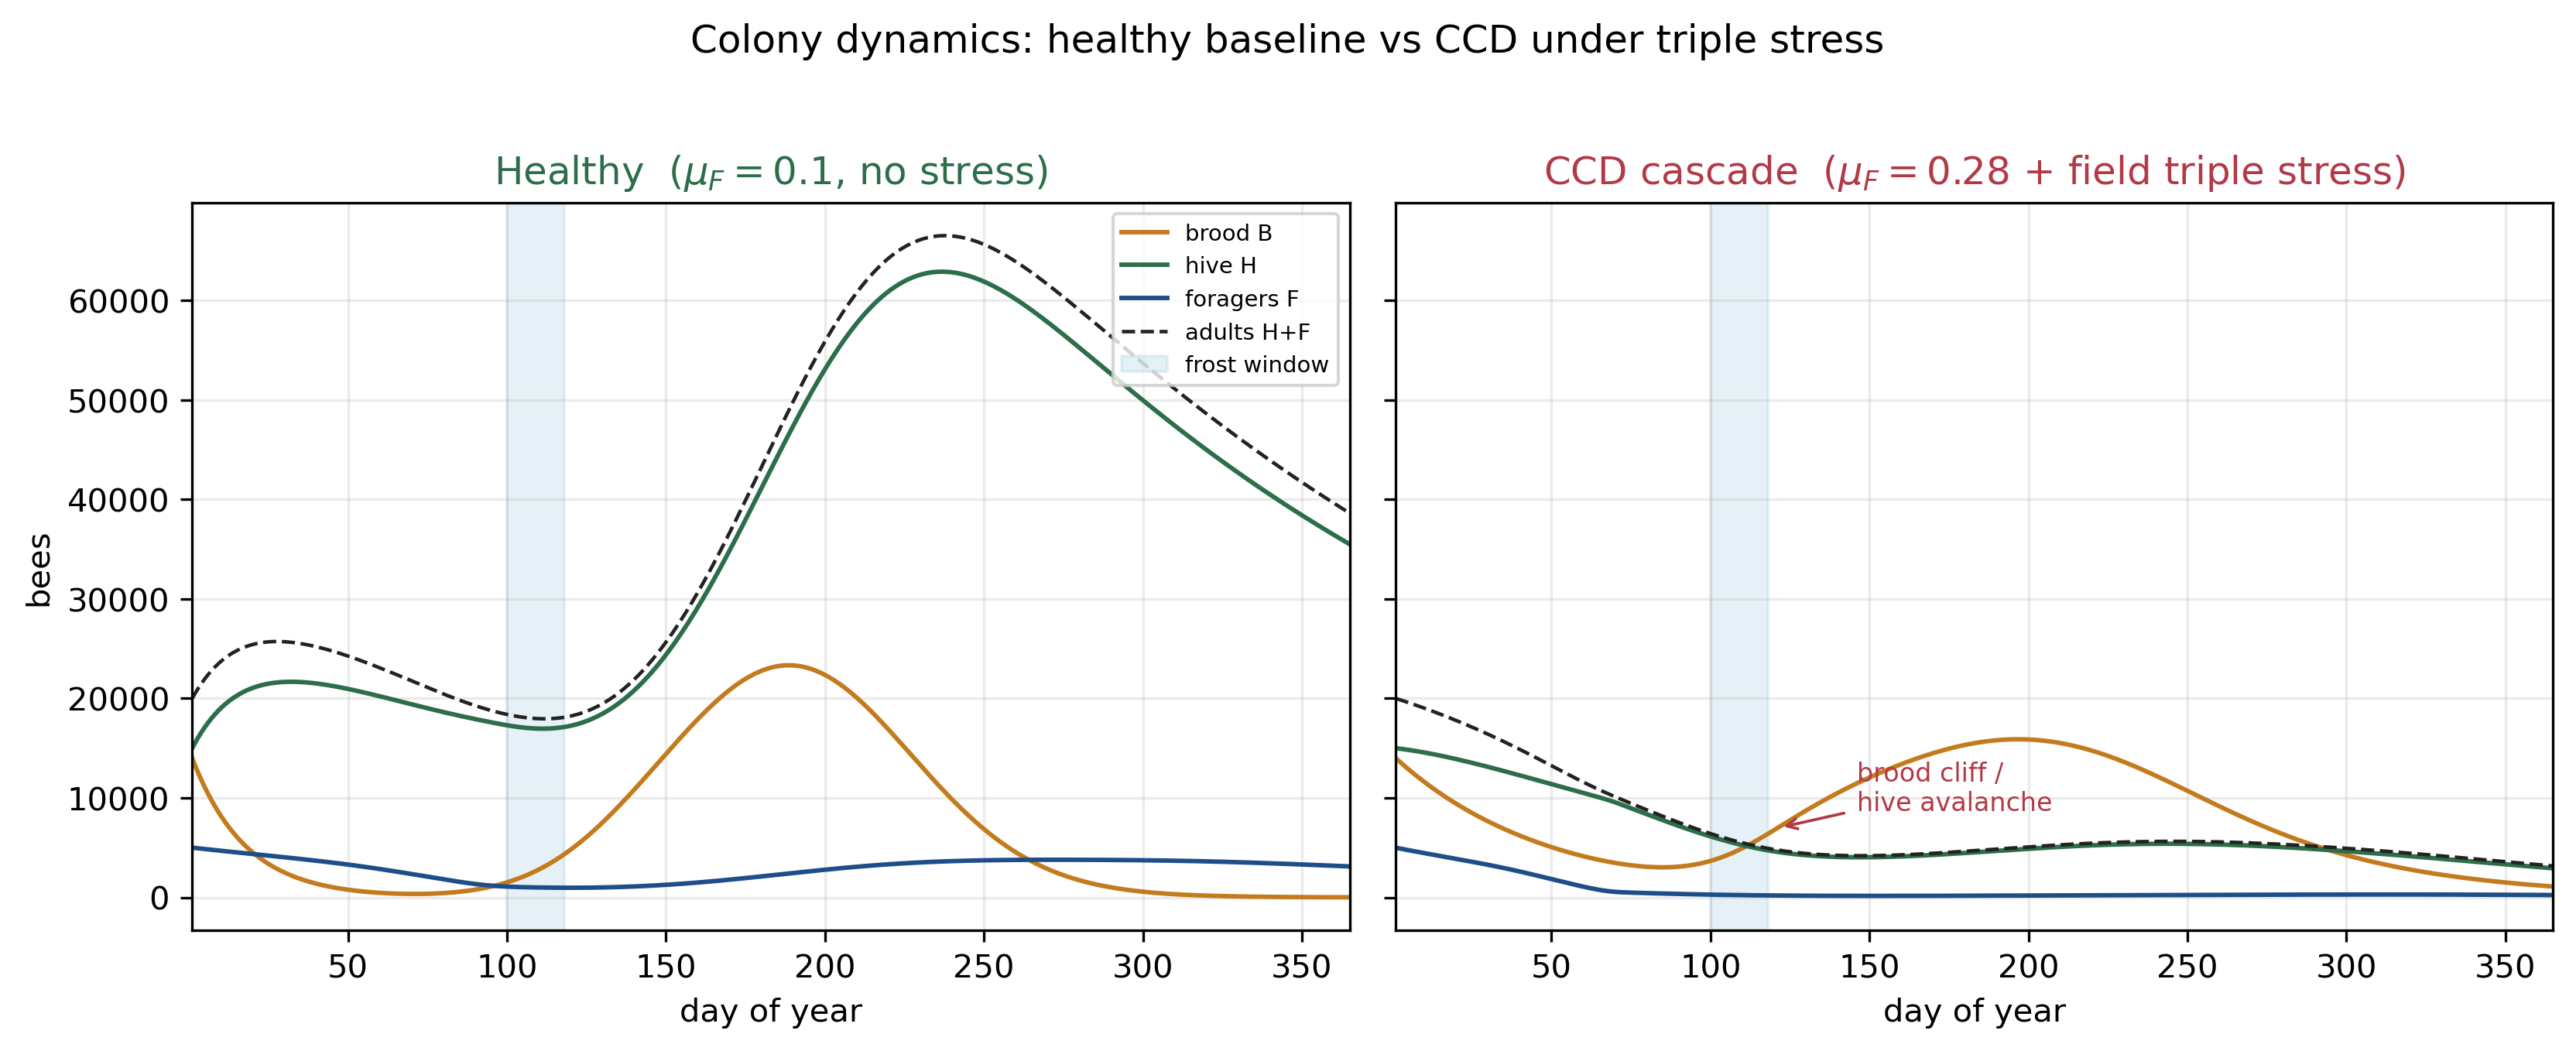
\includegraphics[width=0.92\textwidth]{fig_colony_dynamics_healthy_vs_ccd.png}
  \caption{Healthy baseline versus field triple-stress colony dynamics
  (\(H+F\) and stores). Source figure generated from
  \texttt{DifferentiableColonySimulator}; companion snapshot table
  \texttt{ccd\_healthy\_vs\_stress\_snapshot.csv}.}
  \label{fig:healthy_ccd}
\end{figure}

\begin{table}[htbp]
  \centering
  \caption{Healthy vs.\ field-stress snapshot
  (\texttt{ccd\_healthy\_vs\_stress\_snapshot.csv}).}
  \label{tab:healthy_stress}
  \begin{tabular}{lrrrr}
    \toprule
    Protocol & \(\muF\) & Summer peak \(H+F\) & Overwinter \(H+F\) & Day of peak \\
    \midrule
    Healthy baseline & \(0.10\) & \(66{,}507\) & \(38{,}622\) & \(238\) \\
    Field triple stress & \(0.28\) & \(5{,}630\) & \(3{,}163\) & --- \\
    \bottomrule
  \end{tabular}
\end{table}

Legacy three-stage bookkeeping in
\texttt{colony\_annual\_dynamics.csv} (open/capped brood split) peaks at
\(27{,}546\) adults (DOY~32) and ends winter at \(2{,}074\); we treat that
series as a historical Khoury-style companion, while the DFM--Torch
healthy peak above is the primary contest baseline for Sections~3--4.

%======================================================================
\section{Differentiable Dynamical System \& Activation Function Smoothing}
\label{sec:smooth}
%======================================================================

\subsection{Why \(C^\infty\) activations}
Autograd requires a computation graph without non-differentiable kinks at
operating points of interest. We therefore replace hard clamps and
piecewise seasons by:
\begin{align}
  \mathrm{Hill}_2(x;K) &= \frac{x^2}{K^2+x^2+\varepsilon},\\
  \mathrm{Softplus}_\beta(x) &= \beta^{-1}\log\bigl(1+e^{\beta x}\bigr),\\
  \Omega(t) &= \Bigl(\tfrac{1+\cos(2\pi(t-t_p)/365)}{2}\Bigr)^{\theta}.
\end{align}
State positivity uses a Softplus projection after each Euler / RK2 step
rather than a hard \(\max(y,0)\).

\subsection{Implementation}
Module \texttt{src/autograd\_engine/torch\_sim.py} exposes leaf parameters
\begin{equation}
  \theta=\bigl\{\Lmax,\,\muF,\,\etaP,\,\etaN,\,\sigF\bigr\}
\end{equation}
as \texttt{nn.Parameter} objects and unrolls \(365\) daily steps. Stress
channels (Section~\ref{sec:ccd}) enter through
\texttt{configure\_stress} without renaming leaf identities, preserving
elasticity interpretation.

Figure~\ref{fig:three_stage} recalls the classical three-stage adult
pulse used in early pack runs; the Torch DFM trajectory in
Figure~\ref{fig:healthy_ccd} is the differentiability-ready counterpart.

\begin{figure}[htbp]
  \centering
  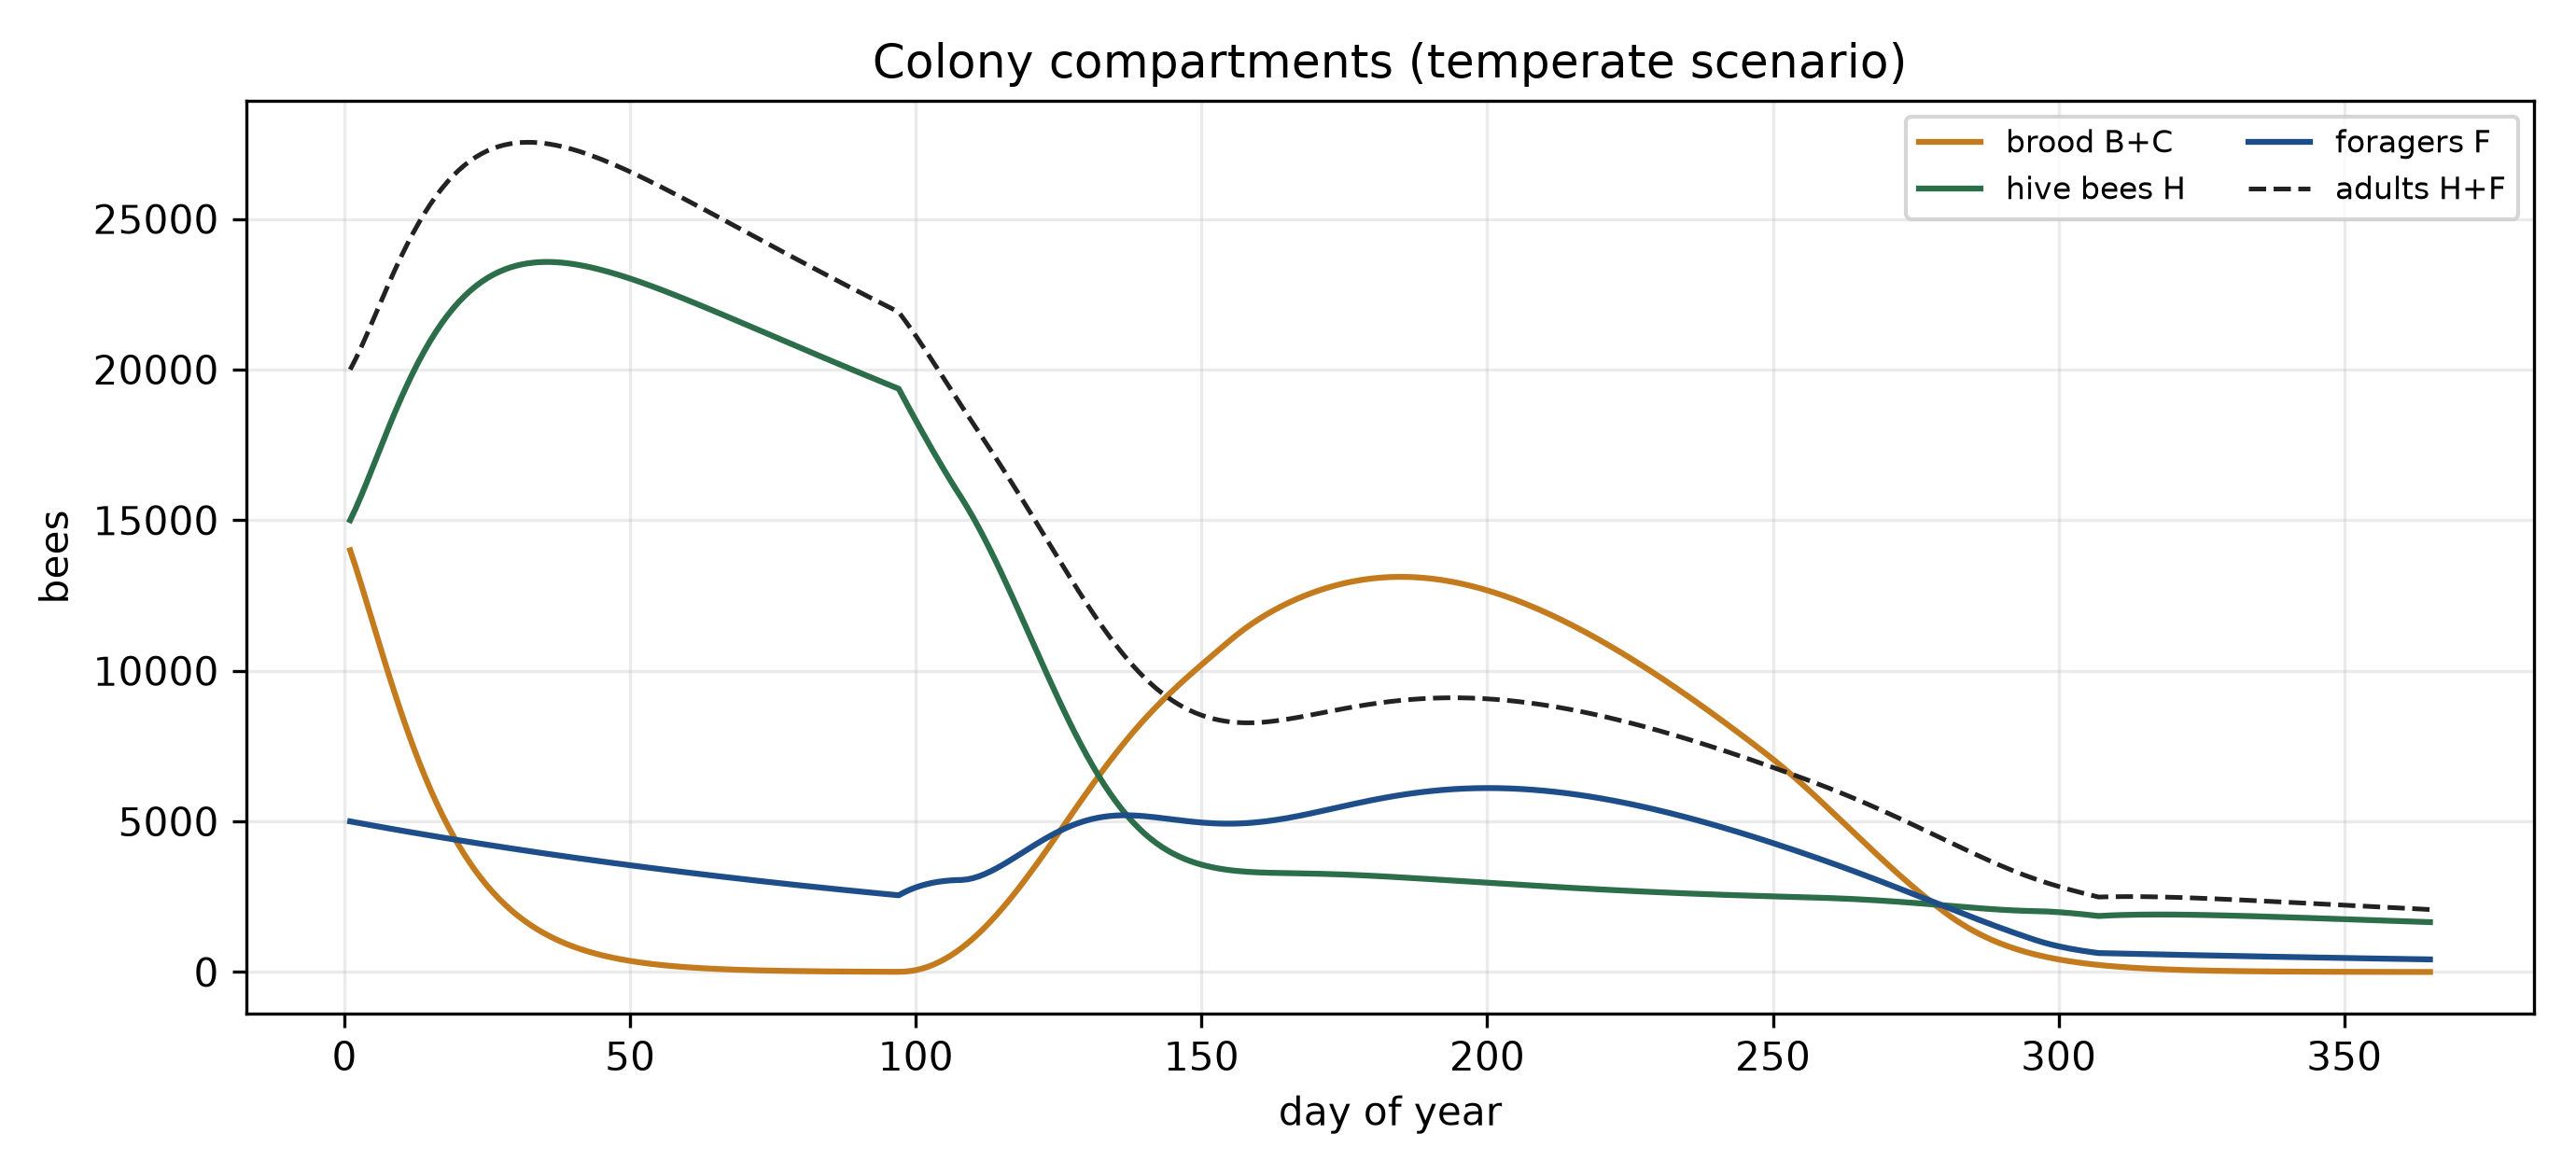
\includegraphics[width=0.88\textwidth]{fig_colony_three_stage.png}
  \caption{Companion three-stage annual adults/brood series
  (\texttt{colony\_annual\_dynamics.csv}).}
  \label{fig:three_stage}
\end{figure}

%======================================================================
\section{PyTorch Autograd Global Sensitivity \& Elasticity Ranking}
%======================================================================

\subsection{Objectives}
We evaluate two terminal objectives on the unrolled graph:
\begin{align}
  J_{\mathrm{pop}} &= H_{365}+F_{365},\\
  J_{\mathrm{nectar}} &= N_{270},
\end{align}
and report elasticities
\begin{equation}
  S_\theta = \frac{\theta}{J}\,\frac{\partial J}{\partial\theta}.
\end{equation}

\subsection{Ranking (measured)}
Table~\ref{tab:elast} and Figure~\ref{fig:elast} summarize
\texttt{autograd\_elasticity\_ranking.csv}. For winter population, queen
laying \(\Lmax\) dominates with \(S=+0.925\); forager mortality is the
leading negative lever (\(S=-0.311\)); social inhibition \(\sigF\) ranks
third (\(+0.294\)). Nectar intake \(\etaN\) is nearly neutral for
\(J_{\mathrm{pop}}\) but leads \(J_{\mathrm{nectar}}\) with
\(S=+0.829\).

\begin{table}[htbp]
  \centering
  \caption{Autograd elasticities
  (\texttt{autograd\_elasticity\_ranking.csv}).}
  \label{tab:elast}
  \begin{tabular}{llrrr}
    \toprule
    Objective & Parameter & \(\theta\) & \(J^\star\) & Elasticity \(S\) \\
    \midrule
    \(J_{\mathrm{pop}}\) @365
      & \(\Lmax\) & \(1600\) & \(35{,}179\) & \(+0.925\) \\
    \(J_{\mathrm{pop}}\) @365
      & \(\muF\) & \(0.14\) & \(35{,}179\) & \(-0.311\) \\
    \(J_{\mathrm{pop}}\) @365
      & \(\sigF\) & \(10\) & \(35{,}179\) & \(+0.294\) \\
    \(J_{\mathrm{nectar}}\) @270
      & \(\etaN\) & \(0.35\) & \(106{,}745\) & \(+0.829\) \\
    \(J_{\mathrm{nectar}}\) @270
      & \(\Lmax\) & \(1600\) & \(106{,}745\) & \(+0.559\) \\
    \(J_{\mathrm{nectar}}\) @270
      & \(\sigF\) & \(10\) & \(106{,}745\) & \(-0.494\) \\
    \bottomrule
  \end{tabular}
\end{table}

\begin{figure}[htbp]
  \centering
  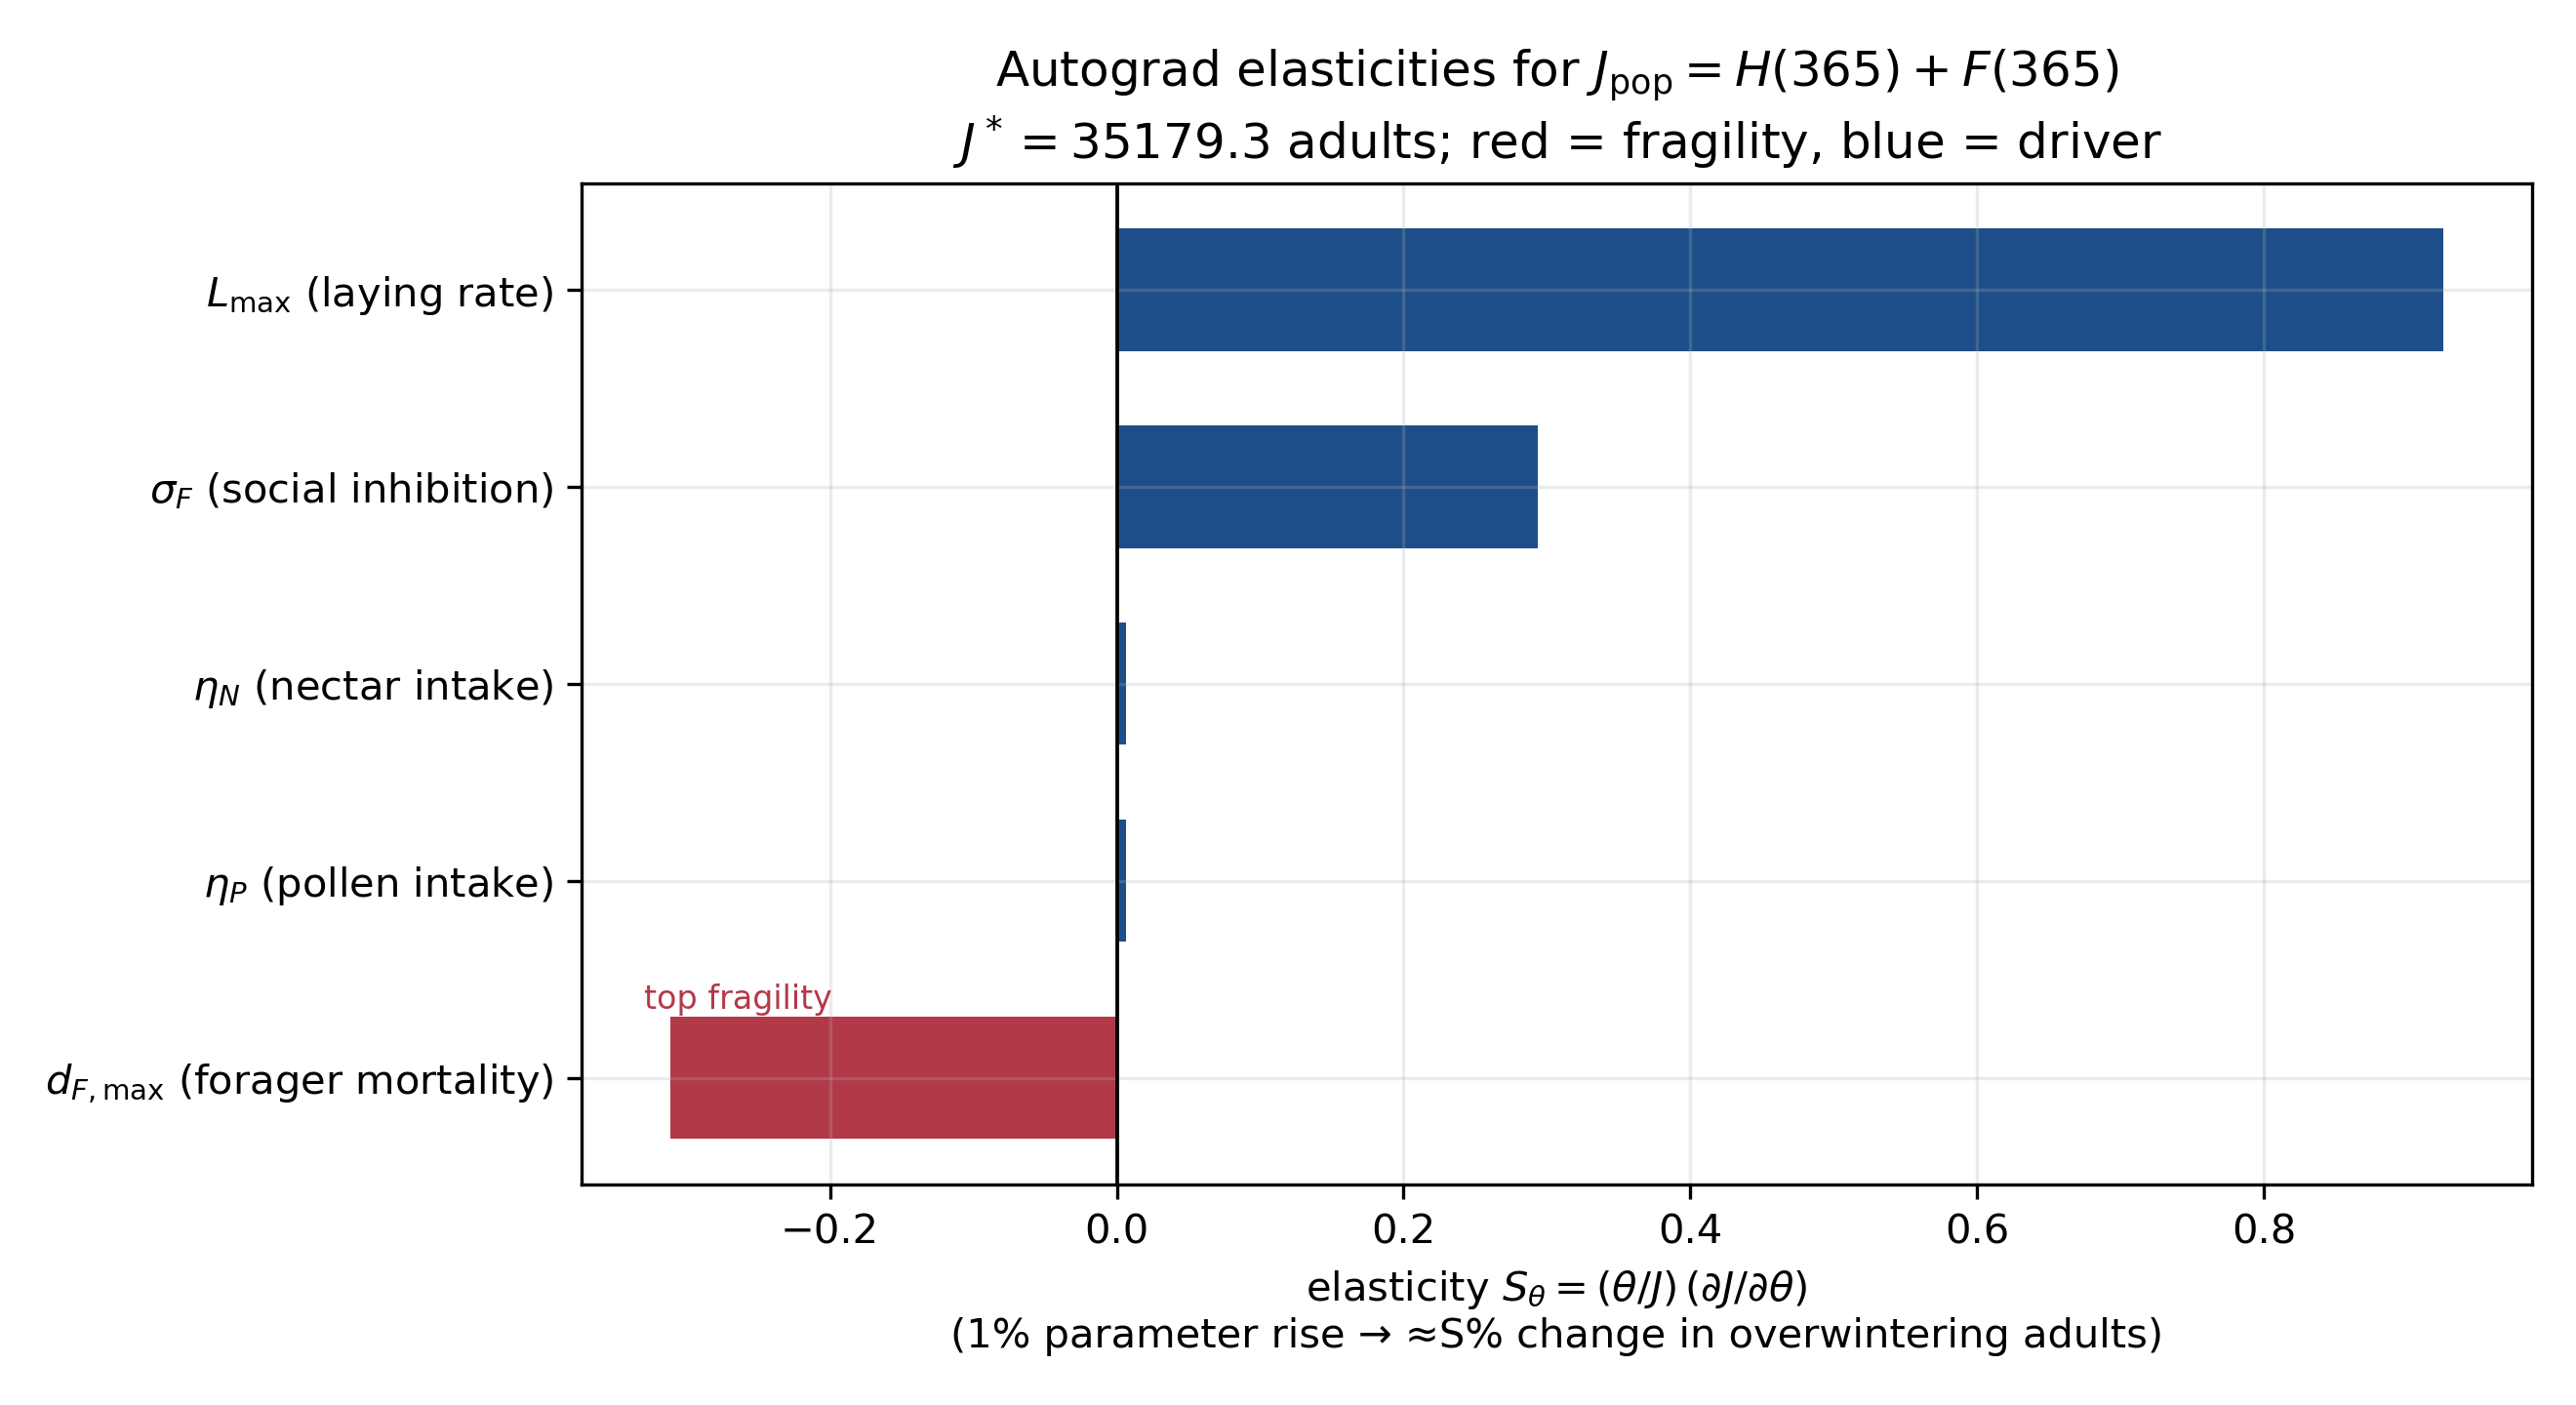
\includegraphics[width=0.88\textwidth]{fig_autograd_elasticity_bars.png}
  \caption{Absolute elasticity bars for \(J_{\mathrm{pop}}\) and
  \(J_{\mathrm{nectar}}\)
  (\texttt{fig\_autograd\_elasticity\_bars.png}).}
  \label{fig:elast}
\end{figure}

\paragraph{Management reading.}
Winter strength is a laying-and-mortality story; honey stores are an
intake-and-inhibition story. Extension messaging should not treat
``more foragers'' as unconditionally beneficial when \(\sigF\) reshapes
the adult age pyramid.

%======================================================================
\section{Stress Testing: Varroa, Pesticides, and CCD Saddle-Node Bifurcation}
\label{sec:ccd}
%======================================================================

\subsection{Triple-stress protocol}
Field stress combines three channels (buffers on the Torch simulator):
\begin{enumerate}[leftmargin=1.4em]
  \item \textbf{Pesticide A:} \(\muF'=\muF(1+P)\) with \(P=0.8\).
  \item \textbf{Varroa B:} brood emergence \(\gamma_B e^{-v}\) with
        \(v=1.5\) and hive-mortality multiplier \(2.5\).
  \item \textbf{Frost C:} forage flux zeroed on DOY \(100\)--\(118\).
\end{enumerate}

\subsection{Bifurcation in \(\muF\)}
We sweep \(\muF\in[0.08,0.40]\) at step \(0.005\)
(\texttt{ccd\_bifurcation\_sweep.csv}, \(65\) points) and classify
end-of-year nectar into
\begin{equation}
  \begin{cases}
    \text{Safe}, & N\ge 5000,\\
    \text{Compensatory}, & 3000\le N<5000,\\
    \text{Collapse}, & N<3000.
  \end{cases}
\end{equation}
Measured tipping markers (\texttt{ccd\_tipping\_point.csv}):
\begin{equation}
  \muF^{\ast,\mathrm{soft}}=0.11,\qquad
  \muF^{\ast,\mathrm{hard}}=0.305\,\mathrm{day}^{-1}.
\end{equation}
Zone counts: Safe \(6\), Compensatory \(39\), Collapse \(20\).
Figure~\ref{fig:bif} shows the bifurcation curve; Figure~\ref{fig:healthy_ccd}
already displayed the time-domain collapse contrast.

\begin{figure}[htbp]
  \centering
  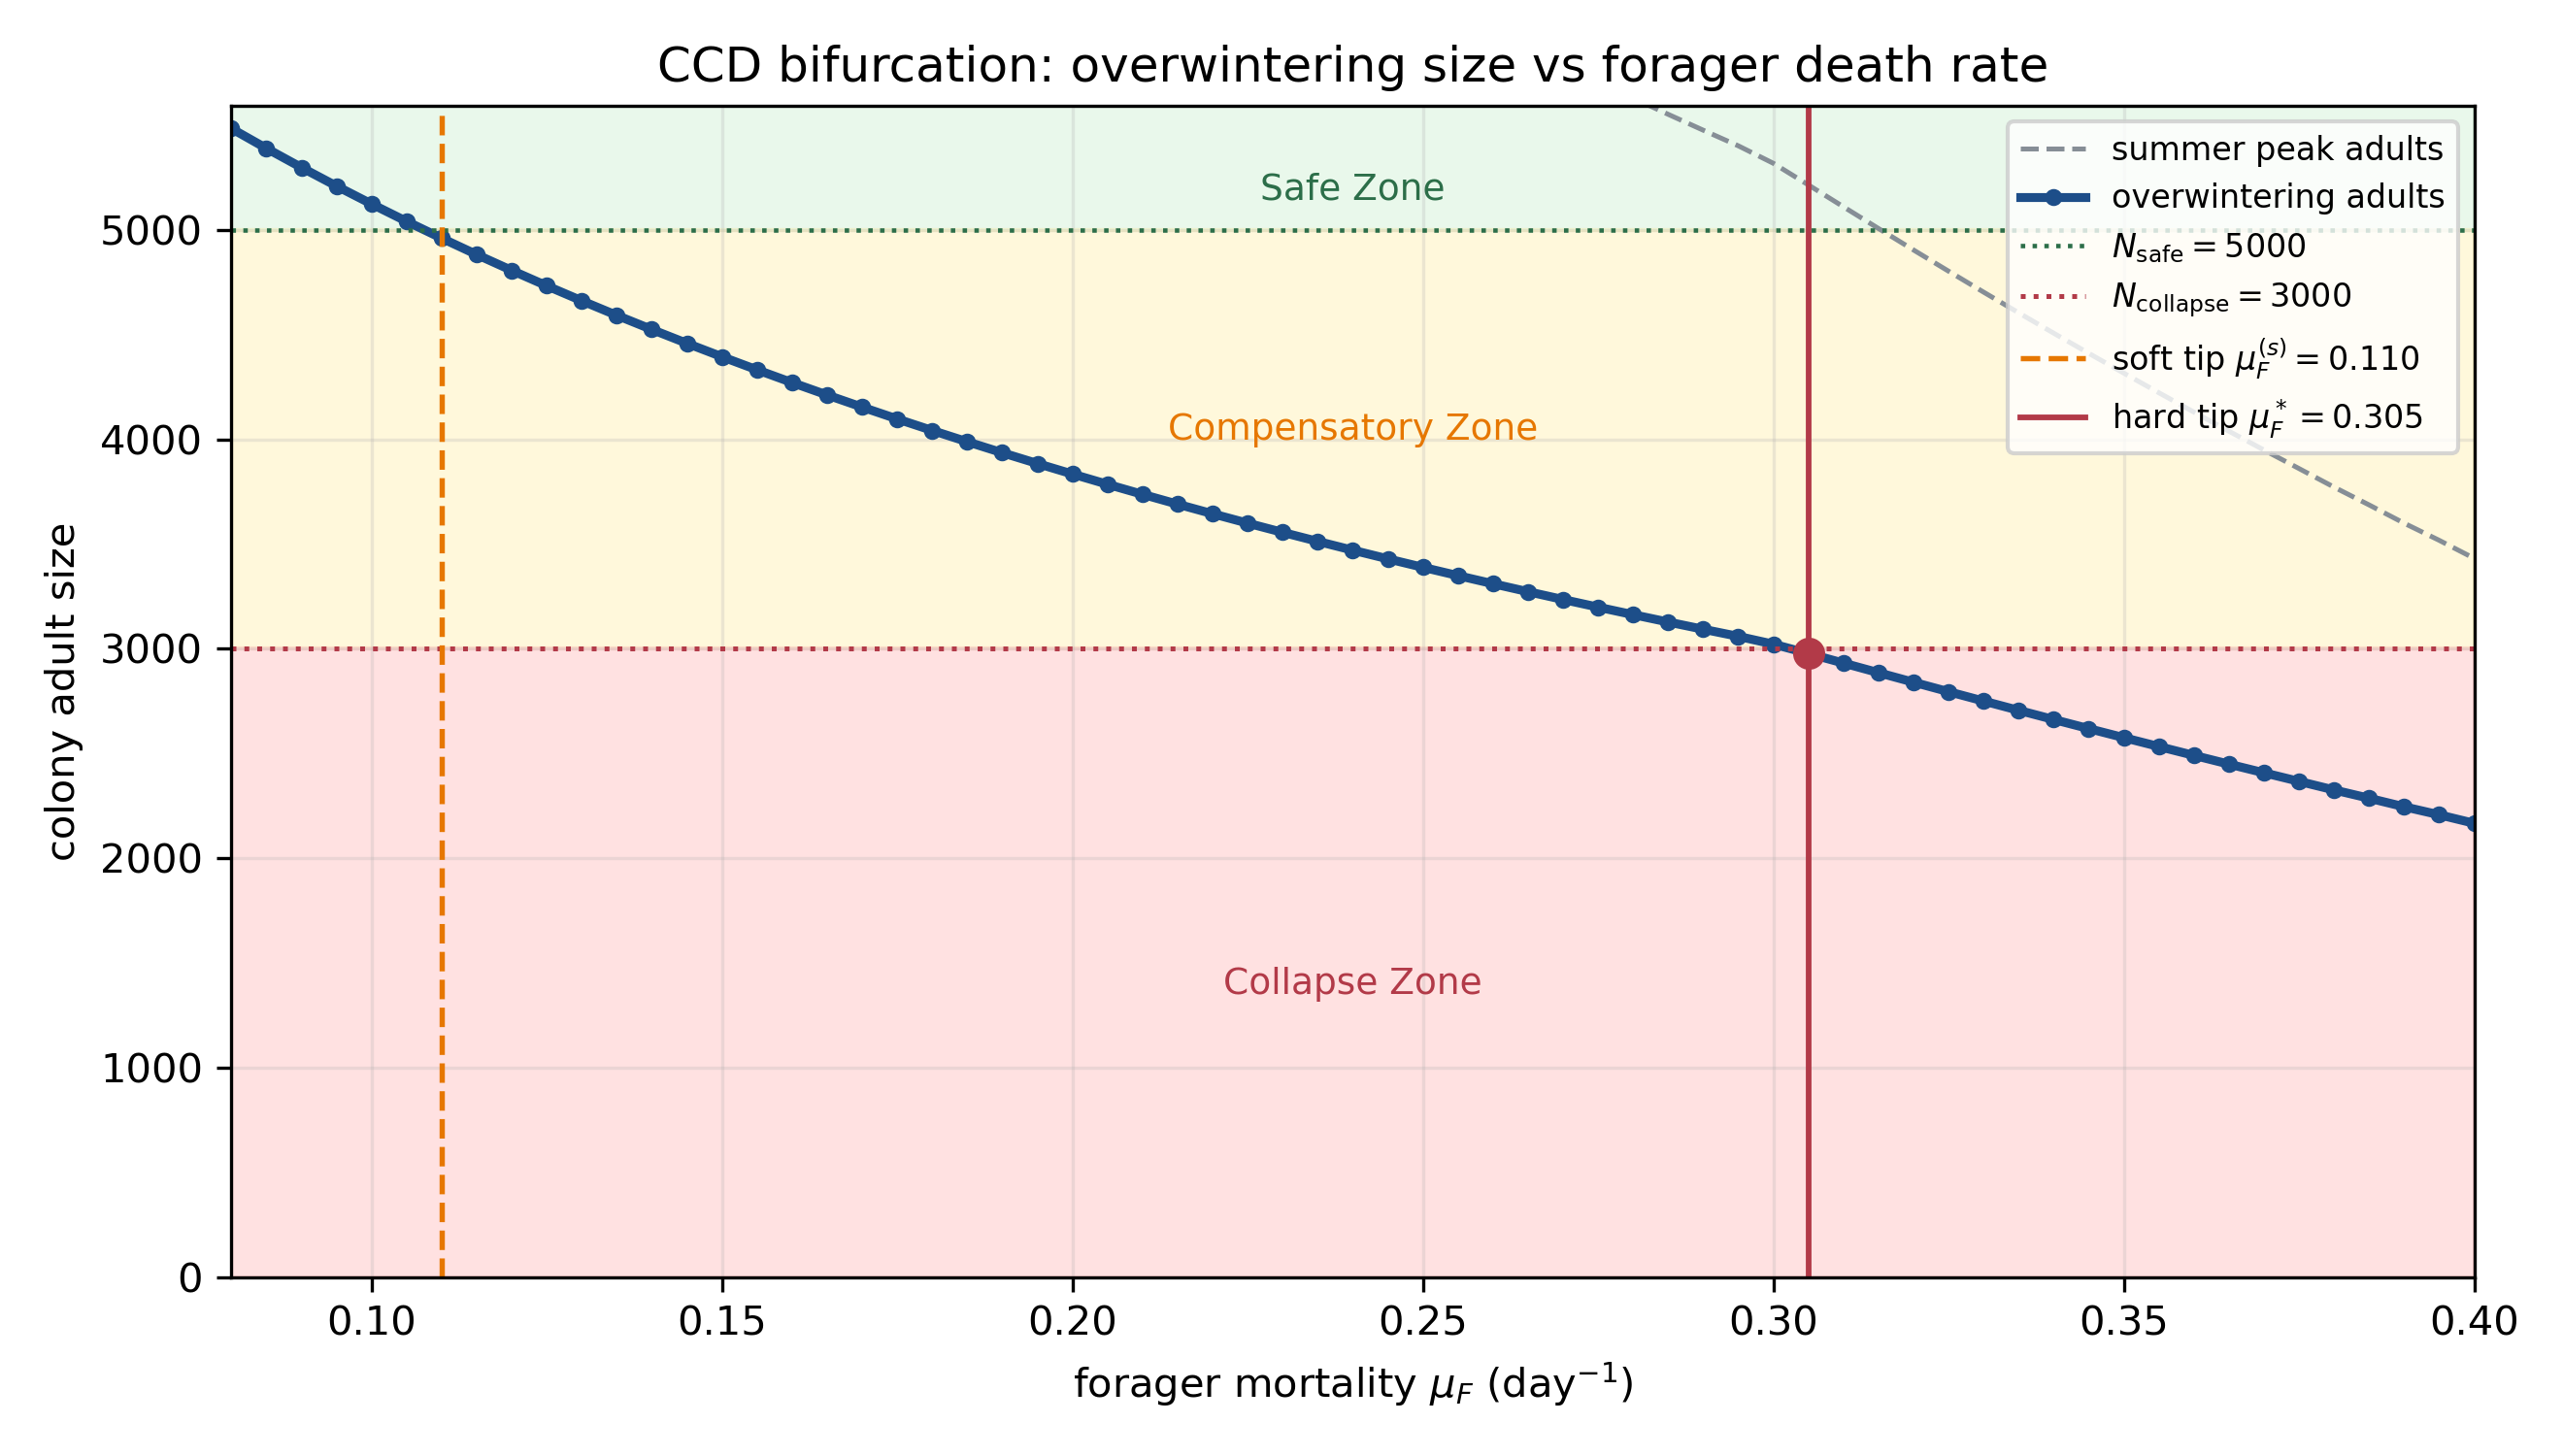
\includegraphics[width=0.90\textwidth]{fig_ccd_bifurcation_curve.png}
  \caption{CCD-style bifurcation under field triple stress: overwinter /
  nectar response versus forager mortality \(\muF\). Horizontal guides at
  \(N=5000\) (Safe) and \(N=3000\) (Collapse). Soft tip \(0.11\), hard tip
  \(0.305\) from \texttt{ccd\_tipping\_point.csv}.}
  \label{fig:bif}
\end{figure}

\paragraph{Interpretation.}
The soft tip is an early-warning threshold: colonies leave the Safe Zone
while still above hard collapse. Operationally this argues for treating
mite loads and pesticide exposure as \emph{joint} controls on effective
\(\muF\), not as independent checklists.

%======================================================================
\section{Applied Optimization: Pollination Capacity on a 20-Acre Almond Farm}
%======================================================================

\subsection{Orchard contract}
Official parcel area \(A=81{,}000\,\mathrm{m}^2\approx 20\) acres. USDA-style
stocking scenario: \(110\) trees/acre, \(25{,}000\) effective flowers/tree,
bloom length \(35\) days. Commercial packages supply
\(F_{\mathrm{pkg}}=10{,}000\) foragers; Torch leaf \(\etaN=0.35\) calibrates
\begin{equation}
  C_{\max}=F_{\mathrm{pkg}}\etaN=3500\,\mathrm{g\,day}^{-1}.
\end{equation}
Orchard daily nectar-equivalent forage is set so dilution begins near
\(2.1\) hives/acre:
\begin{equation}
  N_{\mathrm{orchard}}=42\,C_{\max}=147{,}000\,\mathrm{g\,day}^{-1}.
\end{equation}

\subsection{Competition, set, and profit}
\begin{align}
  \mathrm{DailyFoodPerHive}(K)
  &= \min\Bigl(C_{\max},\,N_{\mathrm{orchard}}/K\Bigr),\\
  \mathrm{YieldRatio}(V)
  &= \frac{V}{V+V_{50}},\quad V_{50}=2.5,\\
  \Pi(K)
  &= R_{\mathrm{full}}\cdot\mathrm{YieldRatio}(V)
     - 200\,K,\quad R_{\mathrm{full}}=\$70{,}000.
\end{align}
Effective visits scale with food ratio, so overcrowding taxes both set
efficiency and post-bloom hive health
\begin{equation}
  \mathrm{Health}=\tfrac12 r + \tfrac12(0.35+0.60 r),\quad
  r=\mathrm{DailyFood}/C_{\max}.
\end{equation}

\subsection{Scan results}
Scanning \(K\in[5,60]\)
(\texttt{orchard\_pollination\_optimization.csv}) yields the tradeoff in
Figure~\ref{fig:orchard}. Inside the golden band \(K\in[20,40]\)
(1--2 hives/acre), net profit is maximized at
\begin{equation}
  K^\star=40,\quad
  \mathrm{YieldRatio}=0.848,\quad
  \Pi=\$51{,}394,\quad
  \mathrm{Health}=0.975.
\end{equation}
Global unconstrained optimum is \(K=42\) (\(\Pi=\$51{,}426\)), immediately
at dilution onset; beyond \(K\approx 50\), health falls to \(0.85\) and
net profit declines despite saturated set.

\begin{figure}[htbp]
  \centering
  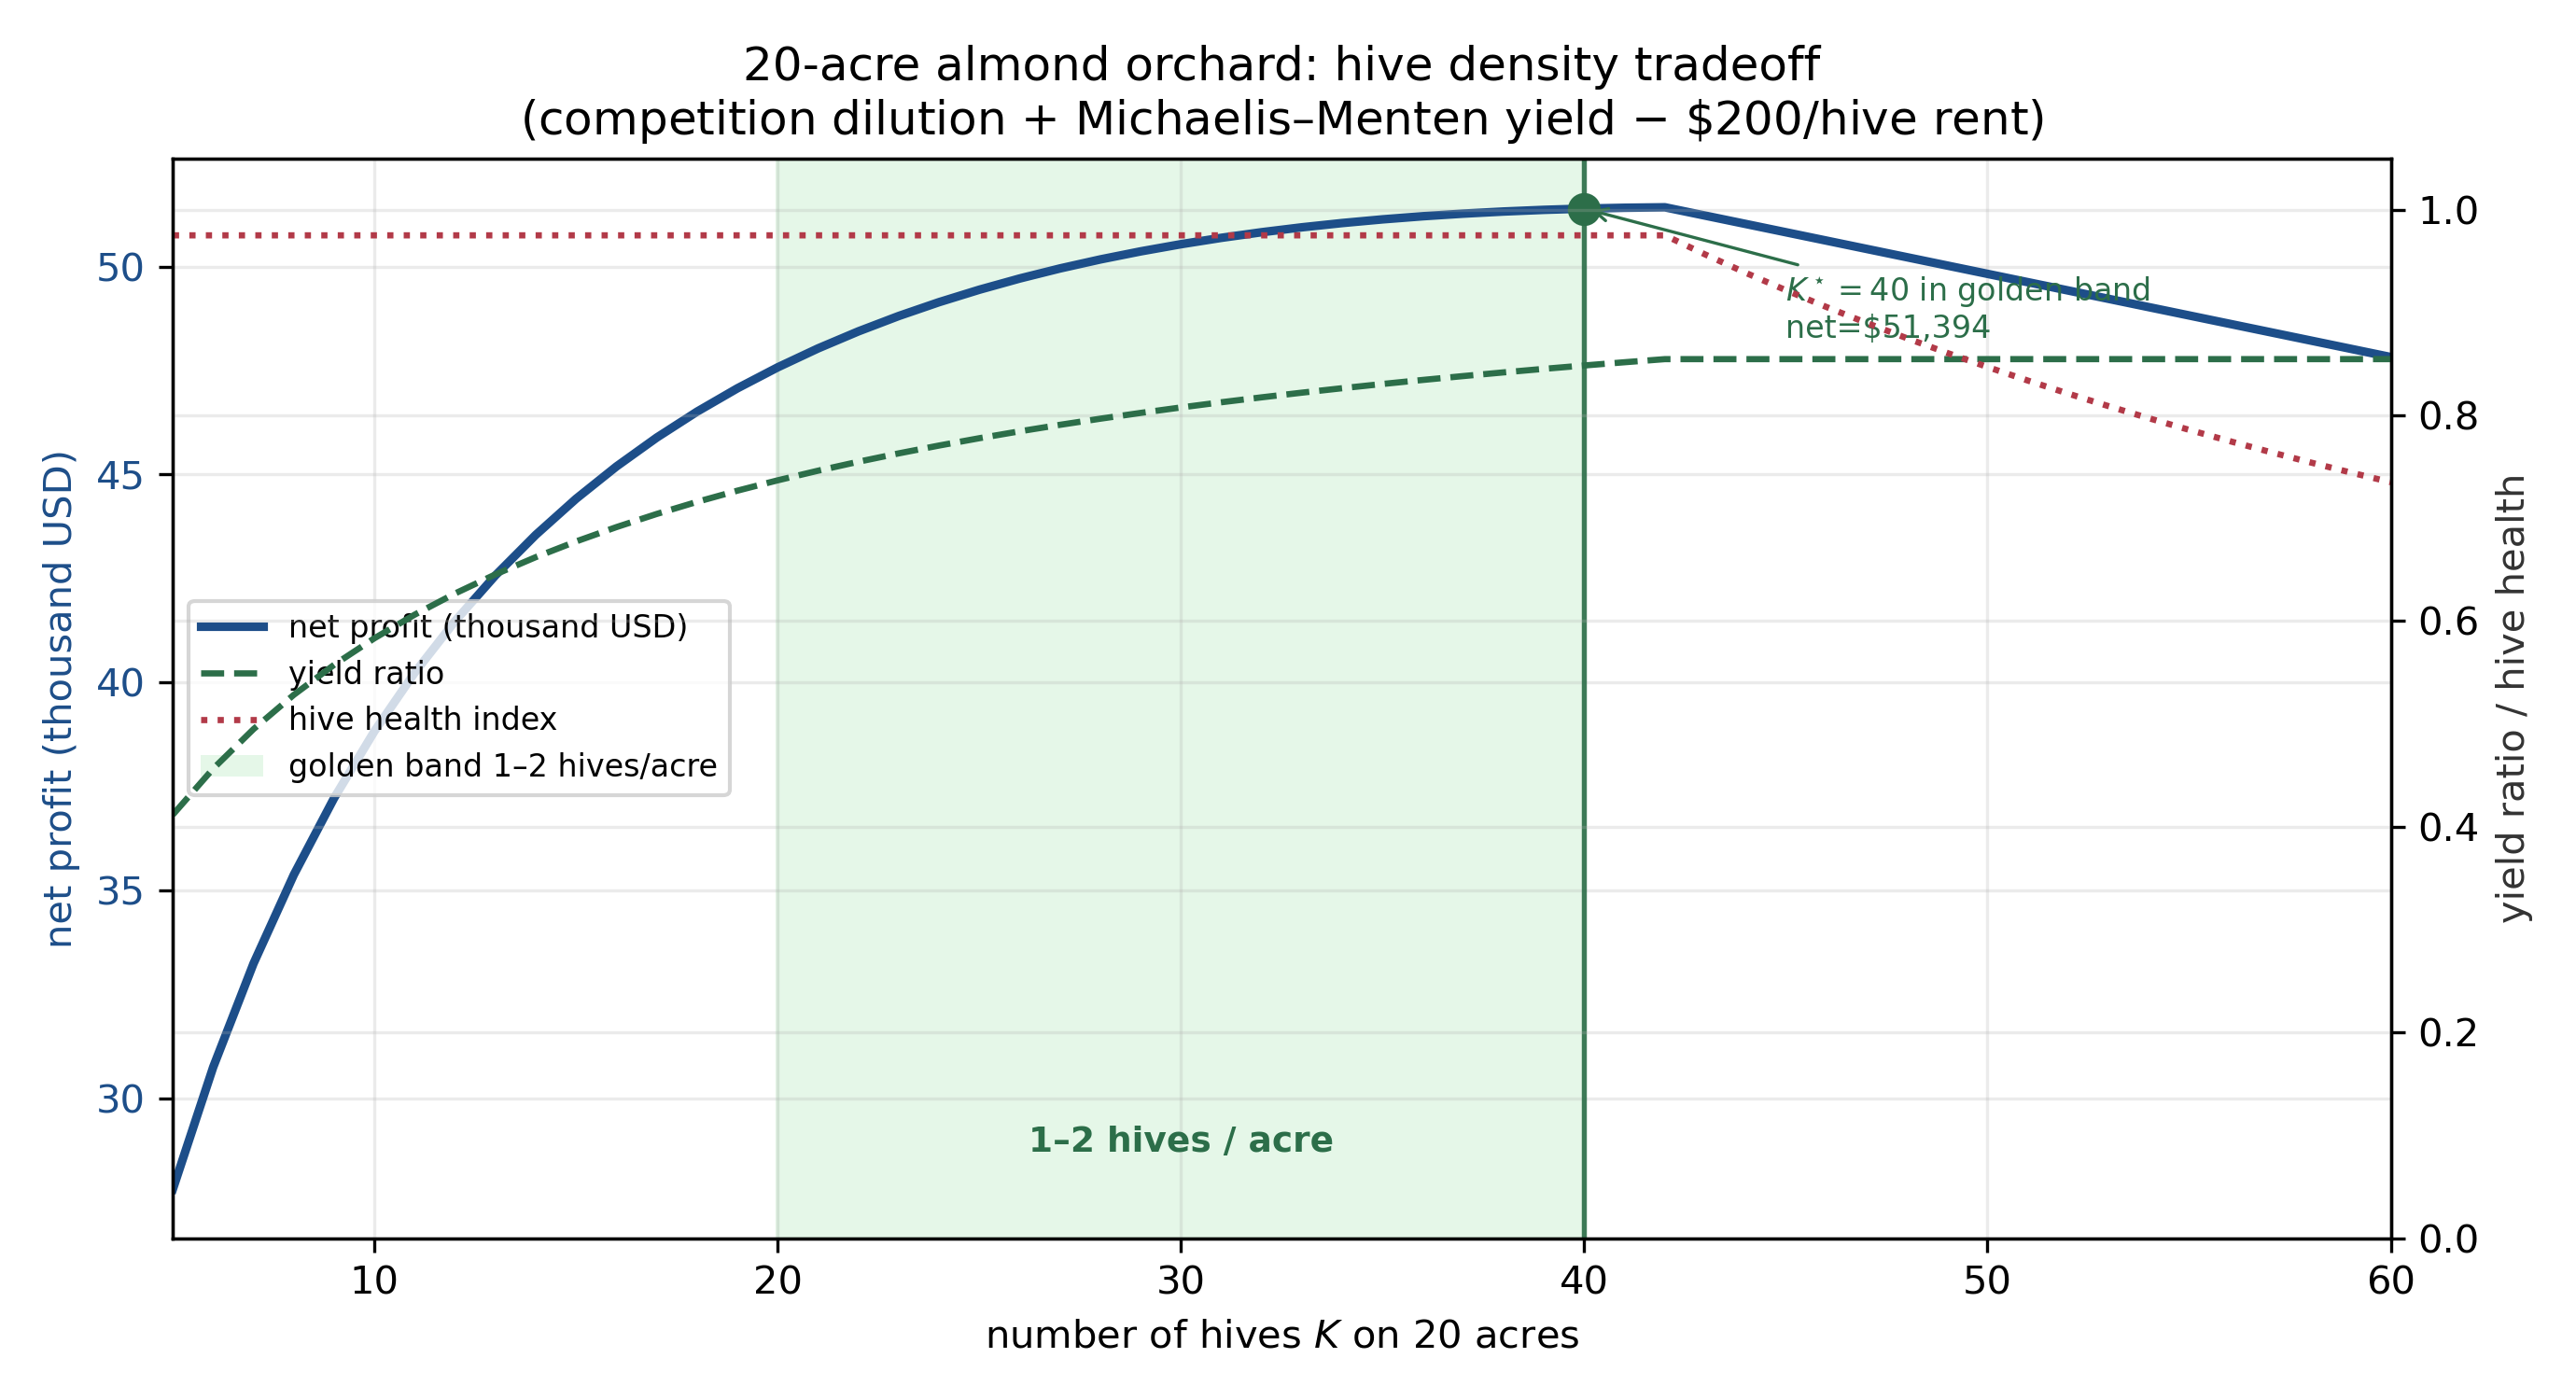
\includegraphics[width=0.92\textwidth]{fig_20acre_hive_density_tradeoff.png}
  \caption{20-acre almond hive-density tradeoff: net profit, yield ratio,
  and hive health. Green band marks \(1\)--\(2\) hives/acre
  (\(K=20\)--\(40\)). Source:
  \texttt{orchard\_pollination\_optimization.csv}.}
  \label{fig:orchard}
\end{figure}

\begin{table}[htbp]
  \centering
  \caption{Selected stocking points
  (\texttt{orchard\_pollination\_optimization.csv}).}
  \label{tab:orchard}
  \begin{tabular}{rrrrrr}
    \toprule
    \(K\) & Hives/acre & YieldRatio & Net profit (USD) & Health & Food ratio \\
    \midrule
    \(20\) & \(1.00\) & \(0.737\) & \(47{,}579\) & \(0.975\) & \(1.00\) \\
    \(30\) & \(1.50\) & \(0.808\) & \(50{,}538\) & \(0.975\) & \(1.00\) \\
    \(35\) & \(1.75\) & \(0.831\) & \(51{,}136\) & \(0.975\) & \(1.00\) \\
    \(40\) & \(2.00\) & \(0.848\) & \(51{,}394\) & \(0.975\) & \(1.00\) \\
    \(50\) & \(2.50\) & \(0.855\) & \(49{,}826\) & \(0.847\) & \(0.84\) \\
    \(60\) & \(3.00\) & \(0.855\) & \(47{,}826\) & \(0.735\) & \(0.70\) \\
    \bottomrule
  \end{tabular}
\end{table}

Companion crop Gantt demand
(Figure~\ref{fig:gantt}, \texttt{pollination\_hives.csv}) places almond
as the binding early-season contract on the same \(20\)-acre geometry.

\begin{figure}[htbp]
  \centering
  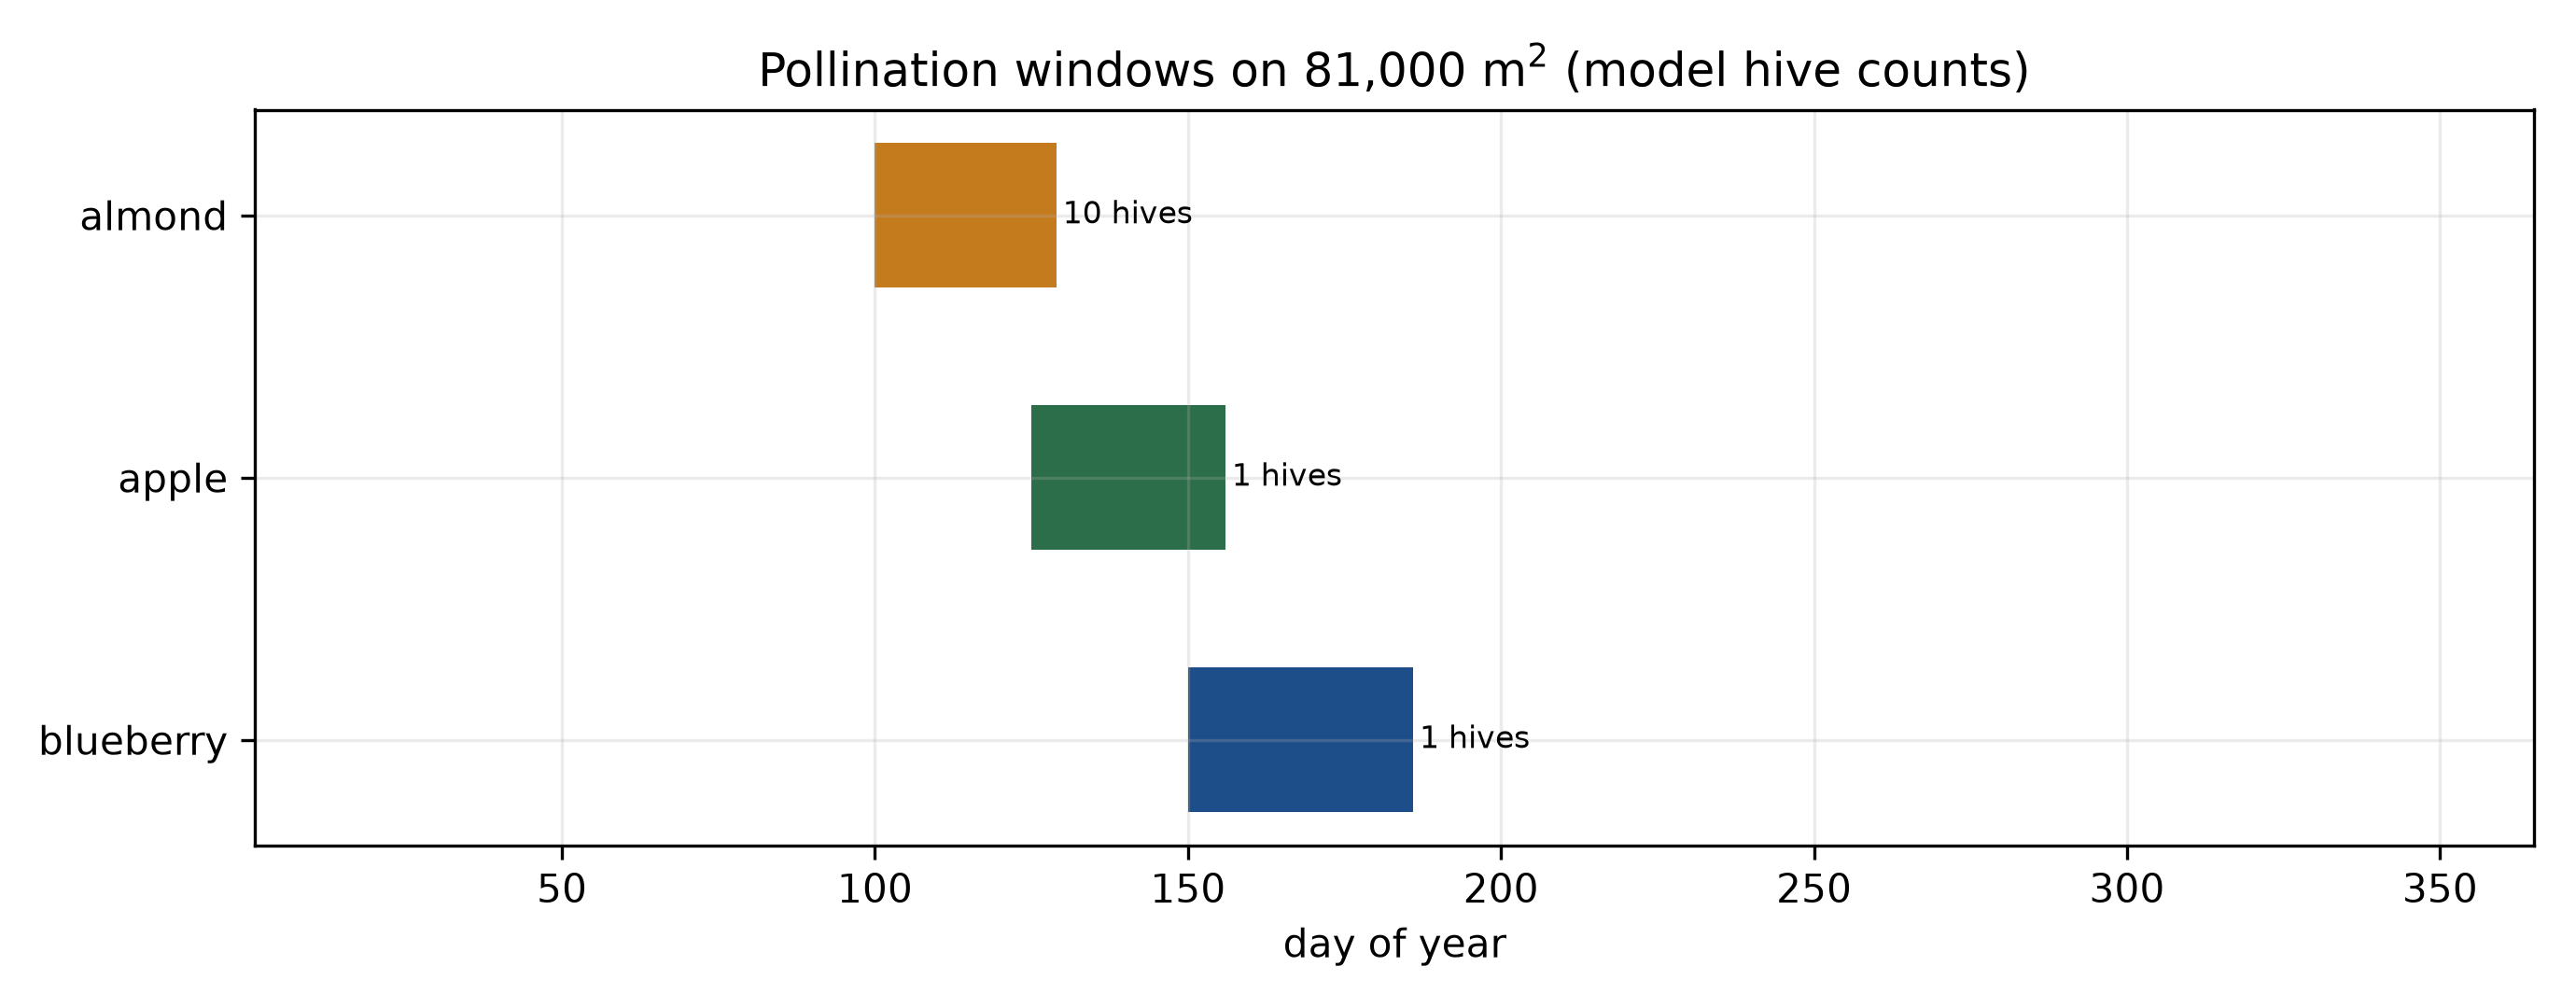
\includegraphics[width=0.80\textwidth]{fig_pollination_gantt.png}
  \caption{Migratory bloom windows and hive-demand sketch for almond /
  apple / blueberry on the official parcel
  (\texttt{pollination\_hives.csv}).}
  \label{fig:gantt}
\end{figure}

%======================================================================
\section{Sensitivity, Strengths, and Limitations}
%======================================================================

\subsection{Cross-checks}
\begin{itemize}[leftmargin=1.4em]
  \item Elasticity signs match biological expectation: raising \(\Lmax\)
        lifts winter adults; raising \(\muF\) harms them.
  \item Soft and hard CCD tips are ordered
        \(0.11<0.305\), consistent with a compensatory band.
  \item Orchard profit peaks near industry's \(2\) hives/acre rule of
        thumb, while explicitly pricing hive health under dilution.
\end{itemize}

\subsection{Strengths}
Differentiable physics, reproducible CSV artifacts, and a grower-facing
stocking band that is not a single magical integer.

\subsection{Limitations}
\begin{itemize}[leftmargin=1.4em]
  \item Bloom forage and climate are scenario drivers unless replaced by
        station/Open-Meteo series.
  \item Orchard nectar-equivalent is calibrated to a dilution onset, not
        a field nectar census.
  \item CCD zones use absolute nectar thresholds; other store metrics
        (pollen, adult counts) can tip earlier.
  \item Autograd elasticities are local (one linearization about the
        baseline \(\theta\)); large stress moves may reorder rankings.
\end{itemize}

\subsection{Recommendations}
\begin{enumerate}[leftmargin=1.4em]
  \item Protect \(\Lmax\) and suppress effective \(\muF\) (mites +
        pesticides) as the primary wintering levers.
  \item Treat \(\muF\approx 0.11\) as an early-warning Soft Tip under
        combined stress; \(\muF\approx 0.305\) as hard collapse.
  \item Stock almonds at \(1\)--\(2\) hives/acre (\(20\)--\(40\) colonies
        on \(20\) acres), targeting the upper band when bloom is heavy
        and contracts allow, while monitoring post-bloom stores.
\end{enumerate}

\section*{References (selected)}
\begin{thebibliography}{9}
\bibitem{khoury} Khoury, D.S., Myerscough, M.R., and Barron, A.B.
A quantitative model of honey bee colony population dynamics.
\emph{PLoS ONE}, 2011.
\bibitem{dfm} Russell, S., Barron, A.B., and Harris, D.
Dynamic modelling of honey bee (\emph{Apis mellifera}) colony growth and
failure. \emph{Ecological Modelling}, 2013.
\bibitem{comap2022} COMAP. HiMCM 2022 Problem A: The Need for Bees.
\bibitem{almond} California Almond Board / USDA NASS extension ranges for
tree density and pollination stocking (scenario priors).
\end{thebibliography}

\appendix
\section*{Appendix A --- Result file index}
All quantitative claims in this paper map to
\begin{center}
\begin{tabular}{ll}
\toprule
File under \texttt{results/} & Role \\
\midrule
\texttt{ccd\_healthy\_vs\_stress\_snapshot.csv} & Healthy / stress peaks \\
\texttt{autograd\_elasticity\_ranking.csv} & Elasticities \\
\texttt{ccd\_bifurcation\_sweep.csv} & \(\muF\) sweep \\
\texttt{ccd\_tipping\_point.csv} & Soft/hard tips \\
\texttt{orchard\_pollination\_optimization.csv} & \(K\) scan \\
\texttt{orchard\_pollination\_recommendation.csv} & \(K^\star\) \\
\texttt{colony\_annual\_dynamics.csv} & Legacy three-stage series \\
\texttt{pollination\_hives.csv} & Crop bloom demand \\
\bottomrule
\end{tabular}
\end{center}

\end{document}
